\documentclass[MASTER.tex]{subfiles}
\begin{document}
%================================================================================================%
\begin{frame}[fragile]
\frametitle{Negative Binomial Regression with \texttt{R}}
\Large
\textbf{PART 3: Negative Binomial Regression}

\bigskip
{
\Large
Negative Binomial Regression is for modeling count outcome variables, when over-dispersion is detected.
}
\end{frame}
%================================================================================================%
\begin{frame}[fragile]
\frametitle{Negative Binomial regression with \texttt{R}}
\large	
\begin{itemize}
		\item Negative binomial regression can be used for over-dispersed count data, that is when the conditional 
		variance exceeds the conditional mean. 
		\[\operatorname{Var}(X) >  \operatorname{E}(X)\]
		\item It can be considered as a generalization of Poisson regression since it has the same mean structure as Poisson 	
		regression and it has an extra parameter (\textit{r}) to model the over-dispersion. 
\end{itemize}
\[\Pr(X = k) = {k+r-1 \choose k} p^k(1-p)^r \quad \mbox{for }k = 0, 1, 2, \dots \]
	
\end{frame}
%================================================================================================%
\begin{frame}[fragile]
\frametitle{Negative Binomial Regression with \texttt{R} }
\large
\textbf{Examples of negative binomial regression}
\begin{itemize}
\item \textbf{Example 1}  School administrators study the attendance behavior of high school juniors at two schools. \\ Predictors of the number of days of absence include the type of program in which the student is enrolled and a standardized test in math.

\item \textbf{Example 2}  A health-related researcher is studying the number of hospital visits in past 12 months by senior citizens in a community based on the characteristics of the individuals and the types of health plans under which each one is covered.
\end{itemize}
\end{frame}
%================================================ %
\begin{frame}[fragile]
\frametitle{Negative Binomial Regression with \texttt{R} }
\Large
\textbf{Description of the data}\\
Let's pursue Example 1 from above.
\begin{itemize}
\item We have attendance data on 314 high school juniors from two urban high schools in the file \textbf{negbin.csv }. 
\item The response variable of interest is days absent, \textbf{\textit{daysabs}}. 
\item The variable \textbf{\textit{math}} gives the standardized math score for each student. 
\item The variable \textbf{\textit{prog}} is a three-level nominal variable indicating the type of instructional program in which the student is enrolled.
\end{itemize}
\end{frame}
%================================================ %
\begin{frame}[fragile]
\frametitle{Negative Binomial Regression with \texttt{R} }
\noindent \textbf{Exploratory Data Analysis}
\begin{verbatim}	
summary(dat)
        id         gender         math         daysabs     
  1001   :  1   female:160   Min.   : 1.0   Min.   : 0.00  
  1002   :  1   male  :154   1st Qu.:28.0   1st Qu.: 1.00  
  1003   :  1                Median :48.0   Median : 4.00  
  1004   :  1                Mean   :48.3   Mean   : 5.96  
  1005   :  1                3rd Qu.:70.0   3rd Qu.: 8.00  
  1006   :  1                Max.   :99.0   Max.   :35.00  
  (Other):308                                              
          prog    
  General   : 40  
  Academic  :167  
  Vocational:107  
\end{verbatim}	
\end{frame}
%===========================================================================%
\begin{frame}
\begin{figure}
\centering
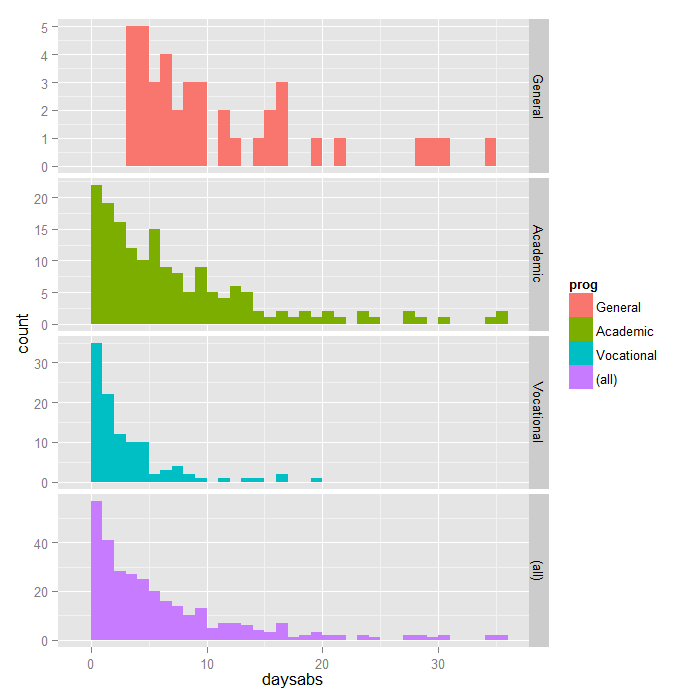
\includegraphics[width=0.85\linewidth]{negbin1}
\end{figure}
Histogram plots showing distribution of the data
\end{frame}
%================================================ %
%\begin{frame}[fragile]
%	\frametitle{Negative Binomial Regression with \texttt{R} }
%	\Large
%
%
%\begin{itemize}
%\item Each variable has 314 valid observations and their distributions seem quite reasonable. 
%\item The unconditional mean of our outcome variable is much lower than its variance.
%\end{itemize}
%
%\end{frame}

\end{document}
